
\section{Experimental area distribution}

The experimental area provided for the operation of the NEXT-DEMO detector is $25m^2$, thus we have assumed a square of 5x5m. In this area we have made the best possible distribution that allow us to have everything in the room and, at the same time, give us enough clearance to move inside the room safely.

Figure \ref{fig:Distribution} shows the proposed distribution of NEXT-DEMO, the magnet, and all the different parts needed for its operation. The details of this distribution need to be discussed with CERN.

\begin{figure}
\centering
%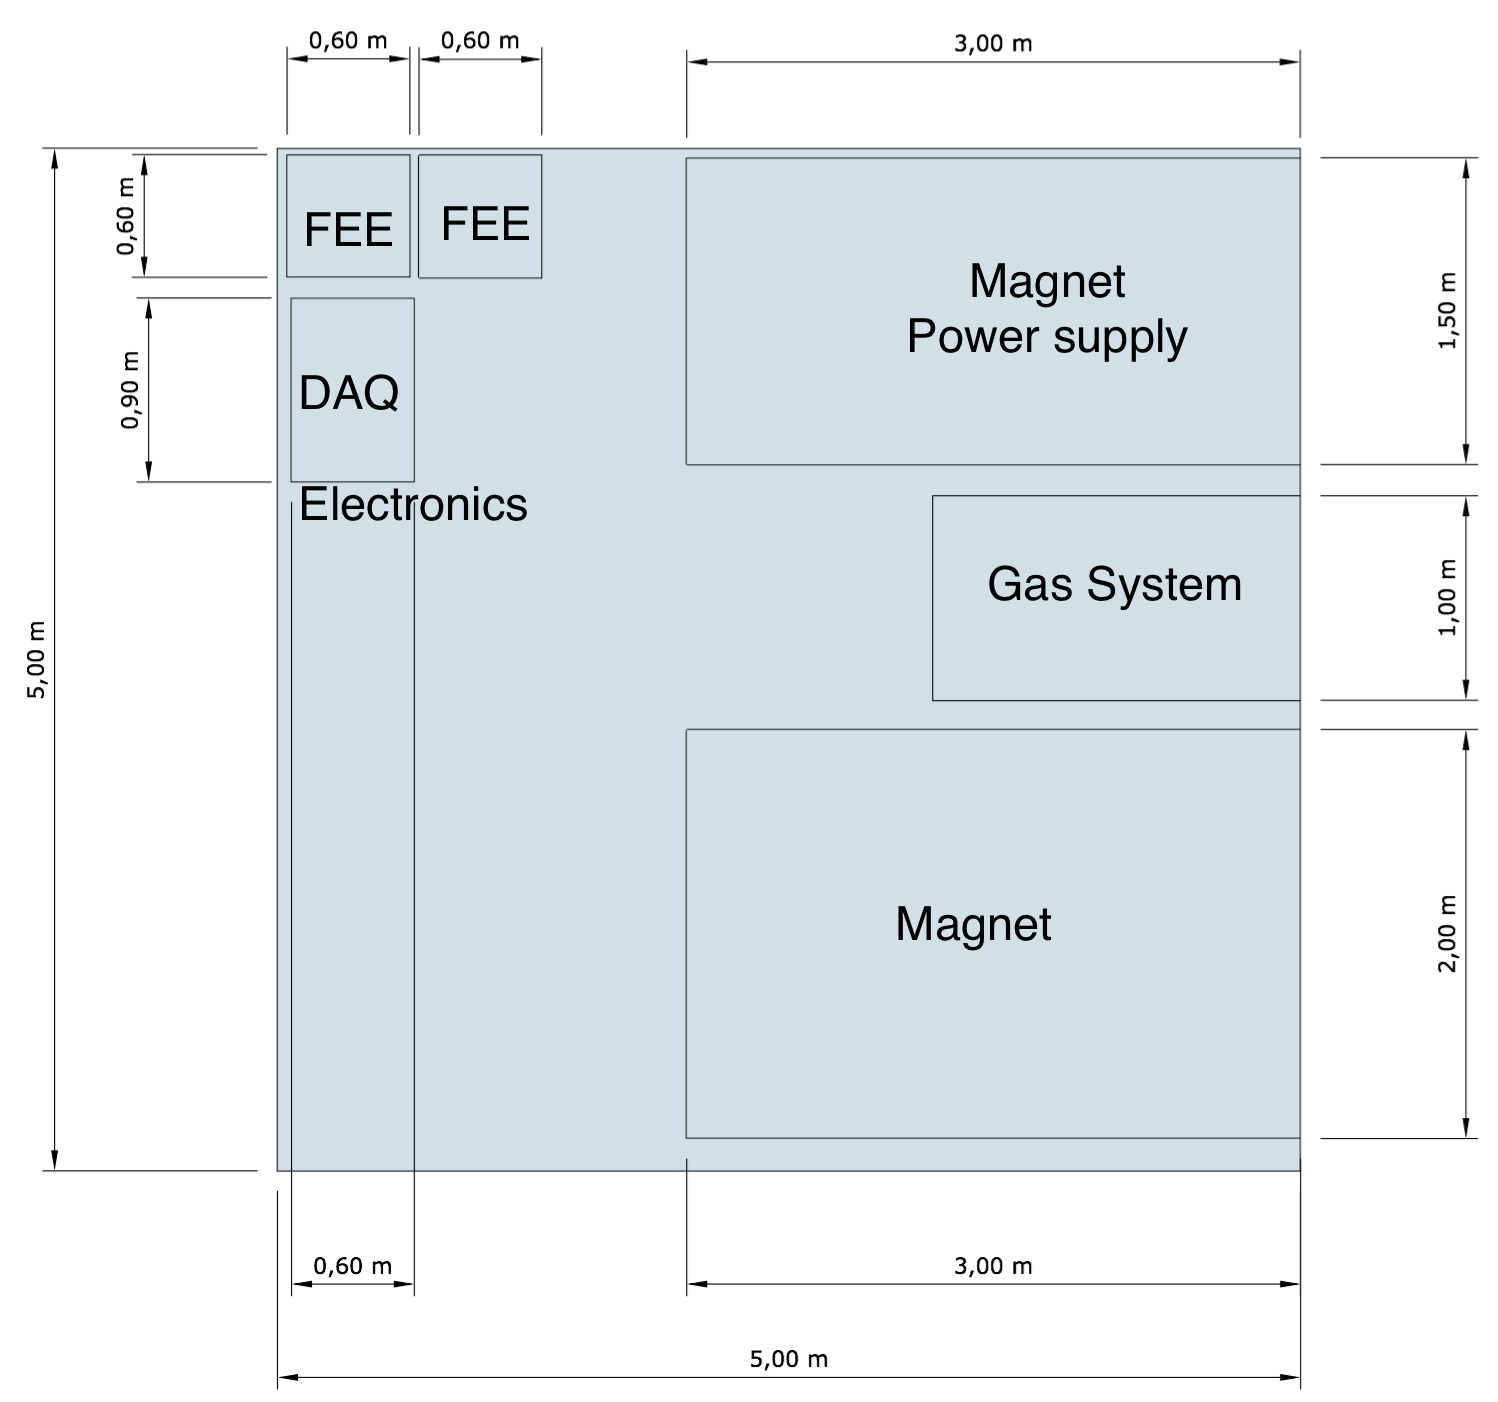
\includegraphics[width=\textwidth]{img/distribution2.png}
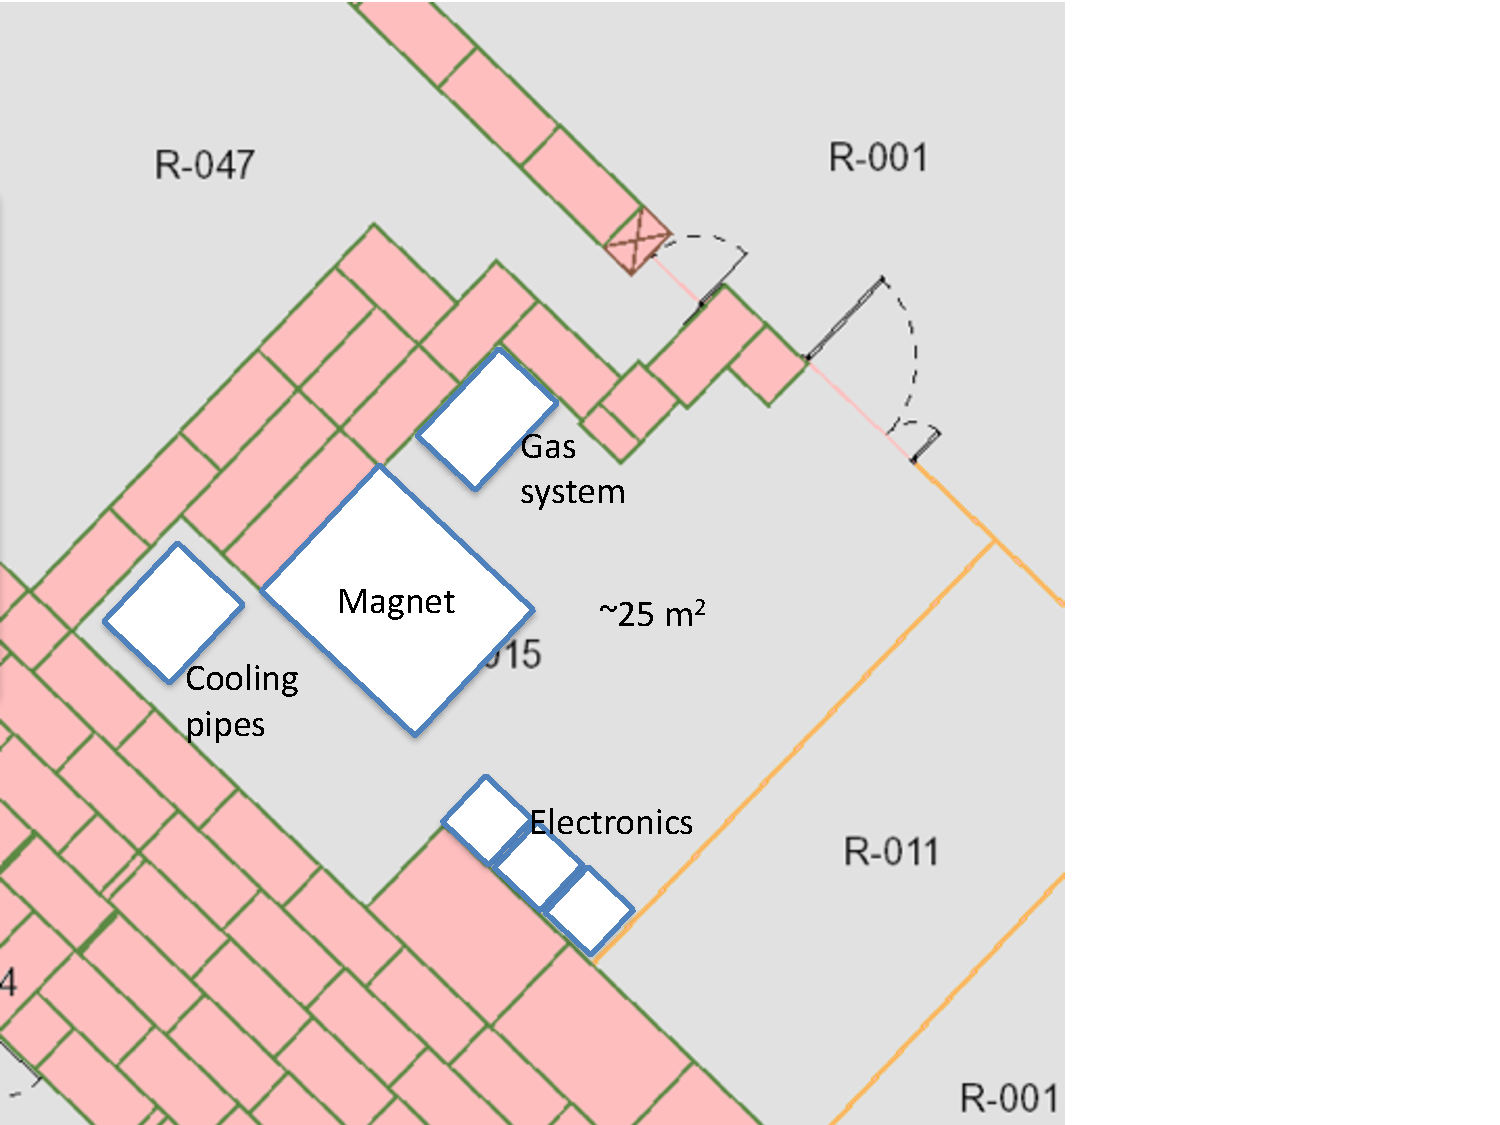
\includegraphics[angle=0,width=\textwidth]{img/distribution_examples.pdf}
\caption{Proposed distribution of the NEXT-DEMO, magnet and all different necessary systems for the operation of the detector in the experimental area} \label{fig:Distribution}
\end{figure}

The blue region will only be used for detector assembly. During detector operation and data taking this region will be free.